\documentclass[preview]{standalone}
\usepackage{amsmath}
\usepackage{tikz}
\usepackage{mathdots}
\usepackage{yhmath}
\usepackage{cancel}
\usepackage{color}
\usepackage{xcolor}
\usepackage{siunitx}
\usepackage{array}
\usepackage{multirow}
\usepackage{amssymb}
\usepackage{gensymb}
\usepackage{tabularx}
\usepackage{extarrows}
\usepackage{booktabs}
\usetikzlibrary{fadings}
\usetikzlibrary{patterns}
\usetikzlibrary{shadows.blur}
\usetikzlibrary{shapes}
\begin{document}
\begin{center}

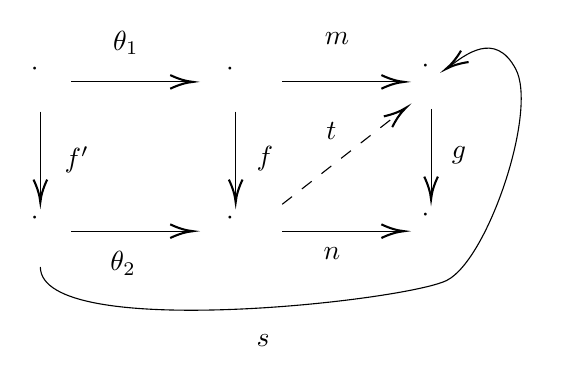
\begin{tikzpicture}[x=0.75pt,y=0.75pt,yscale=-1,xscale=1]
%uncomment if require: \path (0,191); %set diagram left start at 0, and has height of 191

%Straight Lines [id:da8409702886460745] 
\draw    (233.2,34.08) -- (289.92,34.08) ;
\draw [shift={(291.92,34.08)}, rotate = 180] [color={rgb, 255:red, 0; green, 0; blue, 0 }  ][line width=0.75]    (10.93,-3.29) .. controls (6.95,-1.4) and (3.31,-0.3) .. (0,0) .. controls (3.31,0.3) and (6.95,1.4) .. (10.93,3.29)   ;
%Straight Lines [id:da16004951314787053] 
\draw    (334.94,34.08) -- (391.66,34.08) ;
\draw [shift={(393.66,34.08)}, rotate = 180] [color={rgb, 255:red, 0; green, 0; blue, 0 }  ][line width=0.75]    (10.93,-3.29) .. controls (6.95,-1.4) and (3.31,-0.3) .. (0,0) .. controls (3.31,0.3) and (6.95,1.4) .. (10.93,3.29)   ;
%Straight Lines [id:da5842840994613554] 
\draw    (233.2,106) -- (289.92,106) ;
\draw [shift={(291.92,106)}, rotate = 180] [color={rgb, 255:red, 0; green, 0; blue, 0 }  ][line width=0.75]    (10.93,-3.29) .. controls (6.95,-1.4) and (3.31,-0.3) .. (0,0) .. controls (3.31,0.3) and (6.95,1.4) .. (10.93,3.29)   ;
%Straight Lines [id:da7865994793652886] 
\draw    (334.94,106) -- (391.66,106) ;
\draw [shift={(393.66,106)}, rotate = 180] [color={rgb, 255:red, 0; green, 0; blue, 0 }  ][line width=0.75]    (10.93,-3.29) .. controls (6.95,-1.4) and (3.31,-0.3) .. (0,0) .. controls (3.31,0.3) and (6.95,1.4) .. (10.93,3.29)   ;
%Straight Lines [id:da4220078450679592] 
\draw    (218.41,48.46) -- (218.41,90.09) ;
\draw [shift={(218.41,92.09)}, rotate = 270] [color={rgb, 255:red, 0; green, 0; blue, 0 }  ][line width=0.75]    (10.93,-3.29) .. controls (6.95,-1.4) and (3.31,-0.3) .. (0,0) .. controls (3.31,0.3) and (6.95,1.4) .. (10.93,3.29)   ;
%Straight Lines [id:da3145760408714827] 
\draw    (312.53,48.46) -- (312.53,90.09) ;
\draw [shift={(312.53,92.09)}, rotate = 270] [color={rgb, 255:red, 0; green, 0; blue, 0 }  ][line width=0.75]    (10.93,-3.29) .. controls (6.95,-1.4) and (3.31,-0.3) .. (0,0) .. controls (3.31,0.3) and (6.95,1.4) .. (10.93,3.29)   ;
%Straight Lines [id:da5084674615365148] 
\draw    (406.66,47.03) -- (406.66,88.66) ;
\draw [shift={(406.66,90.66)}, rotate = 270] [color={rgb, 255:red, 0; green, 0; blue, 0 }  ][line width=0.75]    (10.93,-3.29) .. controls (6.95,-1.4) and (3.31,-0.3) .. (0,0) .. controls (3.31,0.3) and (6.95,1.4) .. (10.93,3.29)   ;
%Curve Lines [id:da955156656570751] 
\draw    (218.41,123.26) .. controls (218.67,159.3) and (394.61,139.73) .. (414.33,129.67) .. controls (434.05,119.6) and (458.2,47.99) .. (447.44,27.85) .. controls (437.44,9.12) and (422.87,21.28) .. (415.39,26.74) ;
\draw [shift={(413.83,27.85)}, rotate = 326.23] [color={rgb, 255:red, 0; green, 0; blue, 0 }  ][line width=0.75]    (10.93,-3.29) .. controls (6.95,-1.4) and (3.31,-0.3) .. (0,0) .. controls (3.31,0.3) and (6.95,1.4) .. (10.93,3.29)   ;
%Straight Lines [id:da5099104984645619] 
\draw  [dash pattern={on 4.5pt off 4.5pt}]  (334.94,93.05) -- (392.98,47.78) ;
\draw [shift={(394.55,46.55)}, rotate = 142.04] [color={rgb, 255:red, 0; green, 0; blue, 0 }  ][line width=0.75]    (10.93,-3.29) .. controls (6.95,-1.4) and (3.31,-0.3) .. (0,0) .. controls (3.31,0.3) and (6.95,1.4) .. (10.93,3.29)   ;

% Text Node
\draw (212.58,23.6) node [anchor=north west][inner sep=0.75pt]    {$\cdot $};
% Text Node
\draw (212.58,95.52) node [anchor=north west][inner sep=0.75pt]    {$\cdot $};
% Text Node
\draw (306.71,23.6) node [anchor=north west][inner sep=0.75pt]    {$\cdot $};
% Text Node
\draw (306.71,95.52) node [anchor=north west][inner sep=0.75pt]    {$\cdot $};
% Text Node
\draw (400.83,22.17) node [anchor=north west][inner sep=0.75pt]    {$\cdot $};
% Text Node
\draw (400.83,94.08) node [anchor=north west][inner sep=0.75pt]    {$\cdot $};
% Text Node
\draw (252.27,8.22) node [anchor=north west][inner sep=0.75pt]    {$\theta _{1}$};
% Text Node
\draw (250.92,114.66) node [anchor=north west][inner sep=0.75pt]    {$\theta _{2}$};
% Text Node
\draw (354.28,9.22) node [anchor=north west][inner sep=0.75pt]    {$m$};
% Text Node
\draw (353.59,112.78) node [anchor=north west][inner sep=0.75pt]    {$n$};
% Text Node
\draw (415.45,63.88) node [anchor=north west][inner sep=0.75pt]    {$g$};
% Text Node
\draw (321.32,63.88) node [anchor=north west][inner sep=0.75pt]    {$f$};
% Text Node
\draw (228.89,63.88) node [anchor=north west][inner sep=0.75pt]    {$f'$};
% Text Node
\draw (321.32,154.68) node [anchor=north west][inner sep=0.75pt]    {$s$};
% Text Node
\draw (354.94,52.37) node [anchor=north west][inner sep=0.75pt]    {$t$};


\end{tikzpicture}

\end{center}
\end{document}
